\section{Auswahl der Objektdetektoren} \label{detect}

Für das \textit{Smart Warehouse} Szenario soll eine Auswahl zwischen den vier Detektoren \textit{Faster R-CNN}, \textit{Mask R-CNN}, \textit{SSD} und \textit{YOLO} getroffen werden. Als Vergleichsbasis dienen die bereits veröffentlichten Benchmarkergebnisse. Zur Evaluation der Machbarkeitsstudie werden die zuvor eingeführten Bewertungskriterien auf die aus dieser Auswahl resultierenden Objektdetektoren angewendet.

\begin{figure}[ht]
	\begin{center}
		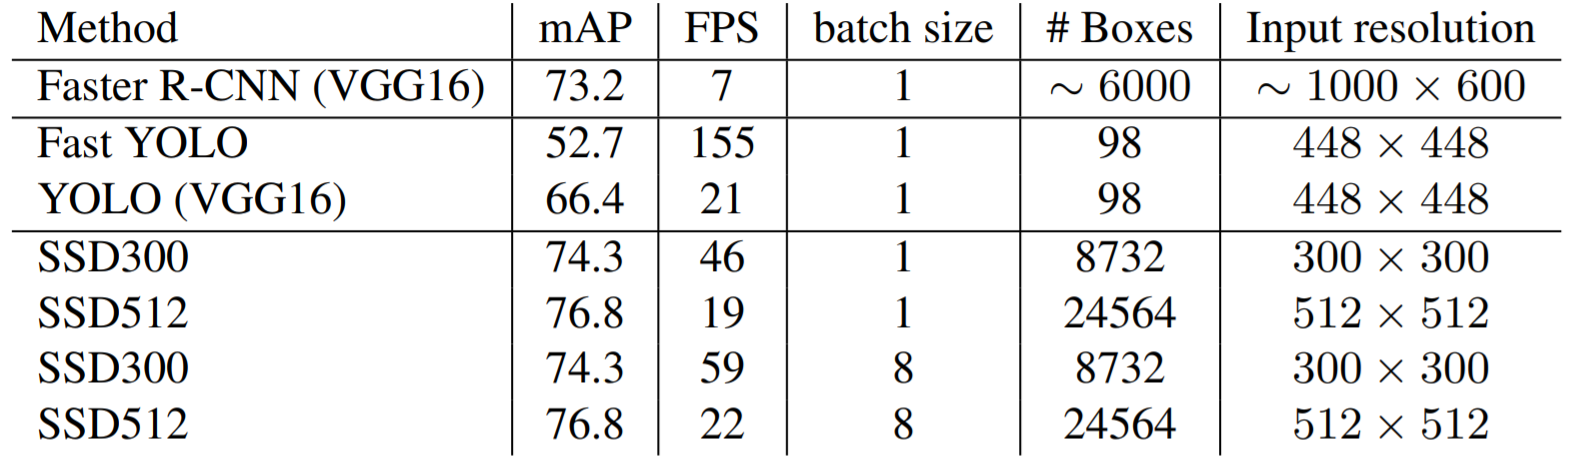
\includegraphics[width=12cm]{Bilder/ssd_results.png} 
		\caption[Vergleich SSD auf PascalVOC 2007]{Vergleich SSD auf PascalVOC 2007\footnotemark \cite{ssd.20161229}}
		\label{result}
	\end{center}
\end{figure}

Abbildung \ref{result} sind die Referenzergebnisse aus der wissenschaftlichen Veröffentlichung des \textit{SSDs} \cite{ssd.20161229}. Die Ergebnisse zeigen, wie die Objektdetektoren \textit{SSD}, \textit{YOLO}, \textit{Fast YOLO} und \textit{Faster R-CNN} untereinander abschneiden\footnotetext{Mask R-CNN wird in der wissenschaftlichen Veröffentlichung von SSD nicht aufgeführt. Beim Vergleich von Faster-RCNN (RoI-Align) mit Mask R-CNN ergibt sich eine mAP von 37.3 zu 38.2 auf Basis des COCO Datensatzes. Die FPS Anzahl betrug wesentlich 5 FPS \cite{KaimingHeGeorgiaGkioxariPiotrDollarRossGirshick.20180224}.}. Jeder der Detektoren besitzt eigene Charakteristika bezüglich der benötigten Auflösung der zu verarbeitenden Bilder, der Anzahl der generierten Bounding Boxen und der Batch Größe während des Trainings. Nach diesen Ergebnissen ist eindeutig festzustellen, dass der \textit{SSD} bezüglich \textit{mAP} mit 74.3\% bzw. 76.8\% am besten abschneidet. \textit{Faster-RCNN} kann zwar mit 73.2\% bezüglich der \textit{mAP} mithalten, ist allerdings mit nur 7 FPS nicht zur schnellen Inferenz ausgelegt. \textit{YOLO} schneidet in beiden Kategorien schlechter als der \textit{SSD} ab, er erzielt wesentlich eine \textit{mAP} von 66.4\% und eine Framerate von 21 FPS. Dem \textit{SSD} gelingt es also, ein gutes Verhältnis zwischen Präzision und Reaktionsvermögen zu bewahren. Durch den Verzicht auf den Schritt der Generierung von Bounding Box Vorschlägen und des \textit{Poolings} kann \textit{SSD} deutlich schneller ablaufen als die Vergleichsdetektoren, während durch das Vordefinieren von Bounding Boxen ebenso eine hohe Präzision erzielt werden kann \cite{ssd.20161229}.

Allerdings ergibt sich vor allem für kleine Objekte ein erschwertes Detektionsvermögen, da diese in den höherliegenden Convolutional Layern untergehen. Als Lösung hierfür kann eine erhöhte Inputgröße gewählt werden (vgl. \textit{SSD512}) oder \textit{Data Augmentation} für den Lernprozess angewandt werden \cite{ssd.20161229}.

Diese Probleme treten bei Netzen der \textit{R-CNN} Familie nicht auf. Wird der \textit{Faster-RCNN} Objektdetektor mit \textit{Mask R-CNN} zur \textit{instanzbasierten Segmentierung} auf Basis des \textit{Common Objects in Context} (COCO) Datensatzes verglichen, so ergibt sich für \textit{Mask R-CNN} mit 38.2\% mAP nur eine geringe Verbesserung gegenüber \textit{Faster R-CNN} mit 37.3\% \cite{KaimingHeGeorgiaGkioxariPiotrDollarRossGirshick.20180224}. Für diesen Benchmark wurde wohlbemerkt das \textit{RoI-Pooling Layer} des \textit{Faster R-CNN} mit einem \textit{RoI-Align Layer} zur besseren Vergleichbarkeit mit dem \textit{Mask R-CNN} Objektdetektor ausgetauscht. Dennoch bleibt auch beim \textit{Mask R-CNN} das Problem eines langsameren Inferenzverhaltens gegenüber dem \textit{SSD} oder \textit{YOLO} offen. Für einen generell industriellen Einsatz könnte dieses langsame Inferenzverhalten möglicherweise problematisch sein, doch für das konkrete Szenario von stehenden Getränkeflaschen in der Machbarkeitsstudie ist eine starke Gewichtung der FPS Metrik zunächst mit Vorsicht zu betrachten \cite{IntanPurnamasar.20181215}. 

Ein weiteres Auswahlkriterium stellt dar, wie gut die Detektoren aufgesetzt und auf eigens erstellte Datensätze umkonfiguriert werden können. Nach Betrachtung mehrerer Repositories ließen sich der \textit{YOLO} und \textit{SSD} Objektdetektor einfach aufsetzen und auf eigene Datensätze anpassen, während bei \textit{Faster R-CNN} und \textit{Mask R-CNN} vermehrt auf Probleme gestoßen wurde. So ist Facebooks Implementierung von \textit{Mask R-CNN} \glqq Detectron\grqq{} beispielsweise nur auf Linux oder macOS lauffähig. Abgeleitete Repositories sind bereits als \textit{deprecated} deklariert und werden nicht mehr gewartet. Ein manuelles Aufsetzen dieser Implementierungen ist nur unter großem Aufwand möglich und wurde aufgrund der limitierten Zeit nicht weiter fortgeführt. Auch die Referenzimplementierung von \textit{Faster R-CNN} ist bereits als \textit{deprecated} deklariert und verweist auf die \textit{Mask R-CNN} Implementierung \textit{Detectron}. Nebenläufige Implementierungen sind ebenso als \textit{Legacy} Implementierungen vermerkt und nur zeitaufwändig manuell aufsetzbar, sofern sie die Windows-Plattform unterstützen.

Aufgrund dieser Umstände und des schlechteren Abschneidens in der zeitkritischen Modellinferenz wurden \textit{YOLO} und \textit{SSD} als die beiden Detektoren ausgewählt, um exemplarisch am \textit{SmartWarehouse Szenario} die Fähigkeit von Objektdetektoren zum industriellen Einsatz zu evaluieren. \textit{YOLO} wird im \textit{Darknet} Framework implementiert, dessen ursprüngliche Variante nicht mehr gewartet wird und zudem keine offizielle Dokumentation für die Verwendung unter Windows bereitsteht. \textit{YOLOv3} besitzt hingegen eine umfassende Dokumentation. \textit{Darknet} lässt sich einfach auf eigene Datensätze anpassen im Gegensatz zur Referenzimplementierung des \textit{SSD} im \textit{Caffe} Frameworks. Aus diesem Grund wurde sich bei \textit{SSD} für eine Custom Implementierung in \textit{PyTorch} entschieden.